\section{Response Time and Output Workload}
\label{app:timing}

Table~\ref{tab:testtiming} and Figure~\ref{fig:testtiming} summarize recorded response times for all ten official-test configurations. The baseline includes 123 joint requests per model, each requesting 17 labels. The stability panel includes 90 requests per condition: three repeats on each of 30 contracts. All attempted requests contribute their observed elapsed time, including invalid or truncated responses and the Gemini Pro request without a recorded answer. These timing summaries therefore describe attempted requests rather than time conditional on a successful answer.

\paragraph{Measurement and comparability.}
All collections use the same client machine, with one in-flight request per model and no automatic retries. The client timer spans the prediction call, including request preparation, connection establishment, network transfer, service-side processing, and response validation. The original seven-model stability collection also times construction of the condition-specific payload; the later three-model extension prepares that payload before starting the timer. Collections occur at different times and retain their provider routes and default caching behavior. Thus, these measurements compare the observed deployments and inference configurations. They do not isolate model computation, equalize hardware or reasoning budgets, or measure maximum throughput. Separate server computation, queueing, and first-token timings were not recorded.

\paragraph{Output workload at fixed visible content.}
Conditions B and C keep all 17 hypotheses visible while requesting one label and 17 labels, respectively. Their comparison changes output workload and structure. Table~\ref{tab:testtiming} reports the median time in each condition and the median of 90 paired elapsed-time differences, matched by contract and repeat. The latter is computed from $t_C-t_B$ for each pair and need not equal the difference between the two condition medians. Its descriptive 95\% intervals resample all three repeats together within each of the 30 contracts, using 5,000 paired bootstrap draws without multiplicity adjustment. Failures remain in these timing pairs.

Jev has the lowest observed baseline median and P95 response times. At fixed visible content, its median changes little when 17 labels are requested instead of one. This small increase is useful for characterizing the service, but does not establish a causal explanation in terms of internal parallelism. Fixed connection and network overhead, caching, and serving policies can also affect how elapsed time changes with output workload. The timing comparison should be read alongside correctness and request validity, rather than as a claim about an isolated model architecture.

\begin{table}[t]
\centering
\footnotesize
\setlength{\tabcolsep}{2.5pt}
\begin{tabularx}{\textwidth}{Xrrrrrr}
\toprule
\rowcolor{tableHeader}
Model & \shortstack{Baseline\\median (s) $\downarrow$} & \shortstack{Baseline\\P95 (s) $\downarrow$} & \shortstack{B: one\\median (s)} & \shortstack{C: 17\\median (s)} & \shortstack{Paired $C-B$\\median (s)} & 95\% CI \\
\midrule
\rowcolor{jevRow}
\modelicon{jev}Jev 1.13.0 & \bestscore{1.24} & \bestscore{1.59} & 1.15 & 1.22 & +0.19 & $[+0.06,+0.24]$ \\
\addlinespace[3pt]
\modelicon{gemini}Gemini 3.5 Flash-Lite & \secondscore{1.60} & 2.78 & 0.99 & 1.86 & +0.49 & $[+0.45,+0.58]$ \\
\modelicon{gemini}Gemini 3.1 Pro Preview & 3.73 & 8.49 & 3.50 & 3.73 & +0.43 & $[-0.05,+0.58]$ \\
\addlinespace[3pt]
\modelicon{openai}GPT-5.6 Luna & 1.74 & \secondscore{2.25} & 1.10 & 1.78 & +0.67 & $[+0.59,+0.71]$ \\
\modelicon{openai}GPT-5.6 Terra & 11.61 & 22.62 & 3.40 & 12.18 & +8.73 & $[+7.73,+9.57]$ \\
\modelicon{openai}GPT-6 Astra & 20.94 & 48.47 & 3.56 & 23.03 & +19.62 & $[+11.90,+28.15]$ \\
\addlinespace[3pt]
\modelicon{claude}Claude Haiku 4.5 & 5.65 & 7.07 & 1.99 & 5.20 & +2.84 & $[+1.06,+3.40]$ \\
\modelicon{claude}Claude Sonnet 5 & 3.27 & 4.51 & 2.32 & 3.25 & +0.84 & $[+0.62,+1.26]$ \\
\addlinespace[3pt]
\modelicon{qwen}Qwen3.5-4B & 86.87 & 175.08 & 25.77 & 82.57 & +56.31 & $[+50.20,+66.03]$ \\
\modelicon{qwen}Qwen3.5-9B & 134.64 & 167.61 & 39.18 & 123.09 & +86.09 & $[+70.99,+94.40]$ \\
\bottomrule
\end{tabularx}
\caption{Client elapsed time for all ten model configurations. The baseline uses 123 contracts with 17 requested judgments per contract. Conditions B and C both show 17 hypotheses and request one or 17 judgments, respectively; each uses 30 contracts and three repeats (90 calls). All attempts, including failures, are retained. Paired changes match contract and repeat; 95\% intervals resample whole contracts 5,000 times. P95 uses linear interpolation. Timings include client, network, and service effects. \textbf{Bold} and \underline{underlining} mark the lowest and second-lowest baseline values, without implying significance.}
\label{tab:testtiming}
\end{table}


\begin{figure}[t]
\centering
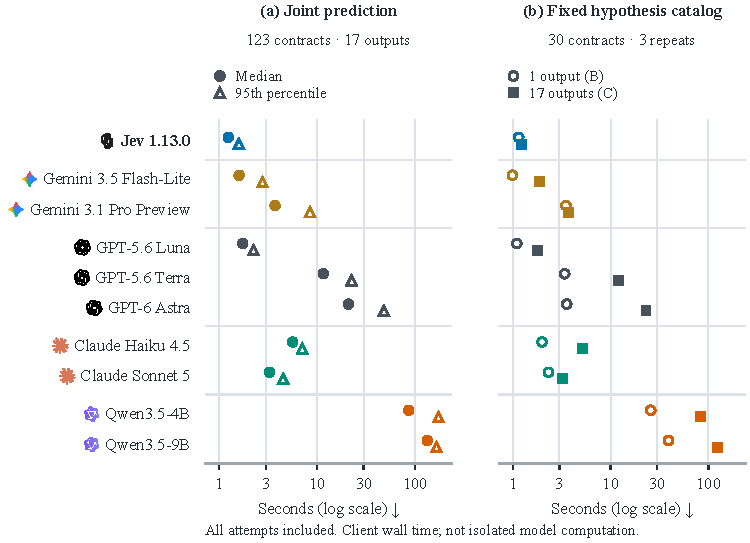
\includegraphics[width=0.90\textwidth]{figures/test_response_time.pdf}
\caption[Jev response time under joint prediction and fixed visible content.]{Jev has the lowest baseline median latency among the tested configurations, with a small additional delay when more judgments are requested. Left: median and 95th-percentile client elapsed time for 123 joint requests per model. Right: median time for requesting one or 17 judgments from the same visible hypothesis catalog (90 requests per condition). All attempts, including invalid responses, are retained. Provider routes and inference settings differ; these measurements do not isolate model computation or establish an architectural cause.
}
\label{fig:testtiming}
\end{figure}
